\documentclass[xcolor=svgnames, english, smaller]{beamer}
\usetheme{Boadilla}
%\usecolortheme[named=Navy]{structure} 

\usepackage[T1]{fontenc}
\usepackage[latin9]{inputenc}
%\setcounter{secnumdepth}{3}
%\setcounter{tocdepth}{3}
\usepackage{amsthm}
\usepackage{amsmath}
\usepackage{graphicx}
\usepackage{xargs}[2008/03/08]
%\usepackage{babel}
\usepackage{subfig}

\makeatletter


%%%%%%%%%%%%%%%%%%%%%%%%%%%%%% Textclass specific LaTeX commands.
 % this default might be overridden by plain title style

\theoremstyle{plain}
\newtheorem{thm}{\protect\theoremname}
\theoremstyle{definition}
\newtheorem{defn}[thm]{\protect\definitionname}
\theoremstyle{plain}
\newtheorem{lem}[thm]{\protect\lemmaname}
\theoremstyle{plain}
\newtheorem{cor}[thm]{\protect\corollaryname}

%%%%%%%%%%%%%%%%%%%%%%%%%%%%%% User specified LaTeX commands.

\makeatother

\providecommand{\corollaryname}{Corollary}
\providecommand{\definitionname}{Definition}
\providecommand{\lemmaname}{Lemma}
\providecommand{\theoremname}{Theorem}

\global\long\def\outify#1{#1^{\text{out}}}
\newcommandx\flowOut[1][usedefault, addprefix=\global, 1=]{\outify{\flow[#1]}}
\global\long\def\Network{\mathscr{N}}
\newcommandx\qdemand[1][usedefault, addprefix=\global, 1=]{r_{#1}}
\newcommandx\flow[1][usedefault, addprefix=\global, 1=]{x_{#1}}
\newcommandx\flowMax[1][usedefault, addprefix=\global, 1=]{\maxify{\flow[#1]}}
\newcommandx\flowIn[1][usedefault, addprefix=\global, 1=]{\inify{\flow[#1]}}
\newcommandx\massmax[1][usedefault, addprefix=\global, 1=]{\mass[#1]^{\max}}
\newcommandx\masscrit[1][usedefault, addprefix=\global, 1=]{\mass[#1]^{\text{crit}}}
\global\long\def\vmass{\vect{\mass}}
\newcommandx\Length[1][usedefault, addprefix=\global, 1=]{\lenCell[#1]}
\newcommandx\cFlow[1][usedefault, addprefix=\global, 1=]{s_{#1}}
\newcommandx\ncFlow[1][usedefault, addprefix=\global, 1=]{t_{#1}}
\newcommandx\parA[1][usedefault, addprefix=\global, 1=]{a_{#1}}
\newcommandx\parB[1][usedefault, addprefix=\global, 1=]{b_{#1}}
\newcommandx\parC[1][usedefault, addprefix=\global, 1=]{c_{#1}}
\global\long\def\coloneqq{:=}
\global\long\def\StackSet{\text{S}(N,r,\beta)}
\global\long\def\BestNashEquilibrium#1#2{\textup{BNE}\left(#1,#2\right)}
\global\long\def\NashEquilibrium#1#2{\textup{NE}\left(#1,#2\right)}
\global\long\def\cffFlow#1#2{\hat{\flow}_{#1}\left(#2\right)}
\newcommandx\opneFlow[3][usedefault, addprefix=\global, 1=]{\bar{\flow}_{#1}^{#2,#3}}
\newcommandx\cffMode[2][usedefault, addprefix=\global, 1=]{\bar{\Mode}_{#1}^{#2}}
\global\long\def\Supp#1{\textup{Supp}\left(#1\right)}
\global\long\def\POS#1#2{\textup{POS}\left(#1,#2\right)}
\global\long\def\Cost#1#2{C_{#1}\left(#1,#2\right)}
\newcommandx\delay[1][usedefault, addprefix=\global, 1=]{D_{#1}}
\newcommandx\lenCell[1][usedefault, addprefix=\global, 1=]{L_{#1}}
\newcommandx\Rea[1][usedefault, addprefix=\global, 1=]{\mathcal{R}^{#1}}
\newcommandx\Routes[1][usedefault, addprefix=\global, 1=]{R_{#1}}
\global\long\def\cellRoute#1#2{\gamma_{#1.#2}}
\global\long\def\odRoute#1#2{\psi_{#1.#2}}
\global\long\def\degradeRatio{}
\newcommandx\mass[1][usedefault, addprefix=\global, 1=]{\rho_{#1}}
\newcommandx\latency[1][usedefault, addprefix=\global, 1=]{l_{#1}}
\global\long\def\Latency{C}
\global\long\def\link{n}
\global\long\def\NLinks{N}
\global\long\def\Graph{G}
\newcommandx\Mode[1][usedefault, addprefix=\global, 1=]{m_{#1}}
\global\long\def\Outgoing{O}
\newcommandx\outCells[1][usedefault, addprefix=\global, 1=]{\Outgoing_{#1}}
\newcommandx\speedFF[1][usedefault, addprefix=\global, 1=]{v_{#1}}
\global\long\def\vff{\speedFF}
\global\long\def\freeflow#1{\speedFF[#1]}
\newcommandx\speedCong[1][usedefault, addprefix=\global, 1=]{w_{#1}}
\global\long\def\minify#1{#1^{\text{min}}}
\global\long\def\maxify#1{#1^{\text{max}}}
\global\long\def\inify#1{#1^{\text{in}}}
\global\long\def\vflow{\vect q}
\global\long\def\vflowMax{\maxify{\vect{\flow}}}
\global\long\def\vflowIn{\inify{\vect{\flow}}}
\global\long\def\vflowOut{\outify{\vect{\flow}}}
\newcommandx\demand[1][usedefault, addprefix=\global, 1=]{\Delta_{#1}}
\newcommandx\dem[1][usedefault, addprefix=\global, 1=]{\demand[#1]}
\newcommandx\supply[1][usedefault, addprefix=\global, 1=]{\Sigma_{#1}}
\newcommandx\supp[1][usedefault, addprefix=\global, 1=]{\supply[#1]}
\global\long\def\fa#1{\forall\,#1}
\global\long\def\fain#1#2{\fa{#1\,\in\,#2}}
\newcommandx\totaltraveltime[1][usedefault, addprefix=\global, 1=]{TTT_{#1}}
\newcommandx\ttt[1][usedefault, addprefix=\global, 1=]{\totaltraveltime[#1]}
\global\long\def\Incoming{I}
\newcommandx\inCells[1][usedefault, addprefix=\global, 1=]{\Incoming_{#1}}
\newcommandx\cell[1][usedefault, addprefix=\global, 1=]{e_{#1}}
\newcommandx\jcn[1][usedefault, addprefix=\global, 1=]{\junction[#1]}
\newcommandx\junction[1][usedefault, addprefix=\global, 1=]{v_{#1}}
\newcommandx\vcell[1][usedefault, addprefix=\global, 1=]{\vect{\cell[#1]}}
\global\long\def\vect#1{\boldsymbol{#1}}
\global\long\def\lonenorm#1{\left|\left|#1\right|\right|_{1}}
\global\long\def\dotT#1#2{\vect{#1^{\mathrm{T}}} \vect{#2} }
\global\long\def\Cells{E}
\global\long\def\Junctions{V}


%###########################################################################################################
\begin{document}

\title{Stackelberg Routing on Horizontal Queueing Networks}
\author{Walid Krichene \and Jack Reilly}
\institute{}
\date{\today}

%---------------------------------------------------------------------------------------------------------------------

\begin{frame}
\titlepage
\end{frame}

%---------------------------------------------------------------------------------------------------------------------
\begin{frame}{Outline}
\tableofcontents
\end{frame}

\AtBeginSubsection[]{
\begin{frame}<beamer>\frametitle{Outline}
\tableofcontents[currentsubsection] 
\end{frame}
}

%###########################################################################################################
\section{Latency Functions}

\subsection{Derivation from Fundamental Diagram}

%---------------------------------------------------------------------------------------------------------------------
\begin{frame}{Assumptions of Fundamental Diagram}
\begin{block}
{Two Modes}
\begin{enumerate}
\item <1->Constant slope in the free-flow mode.
\item <2->Flow is decreasing function of density in congested mode.
\end{enumerate}
\end{block}

\begin{figure}
\begin{centering}
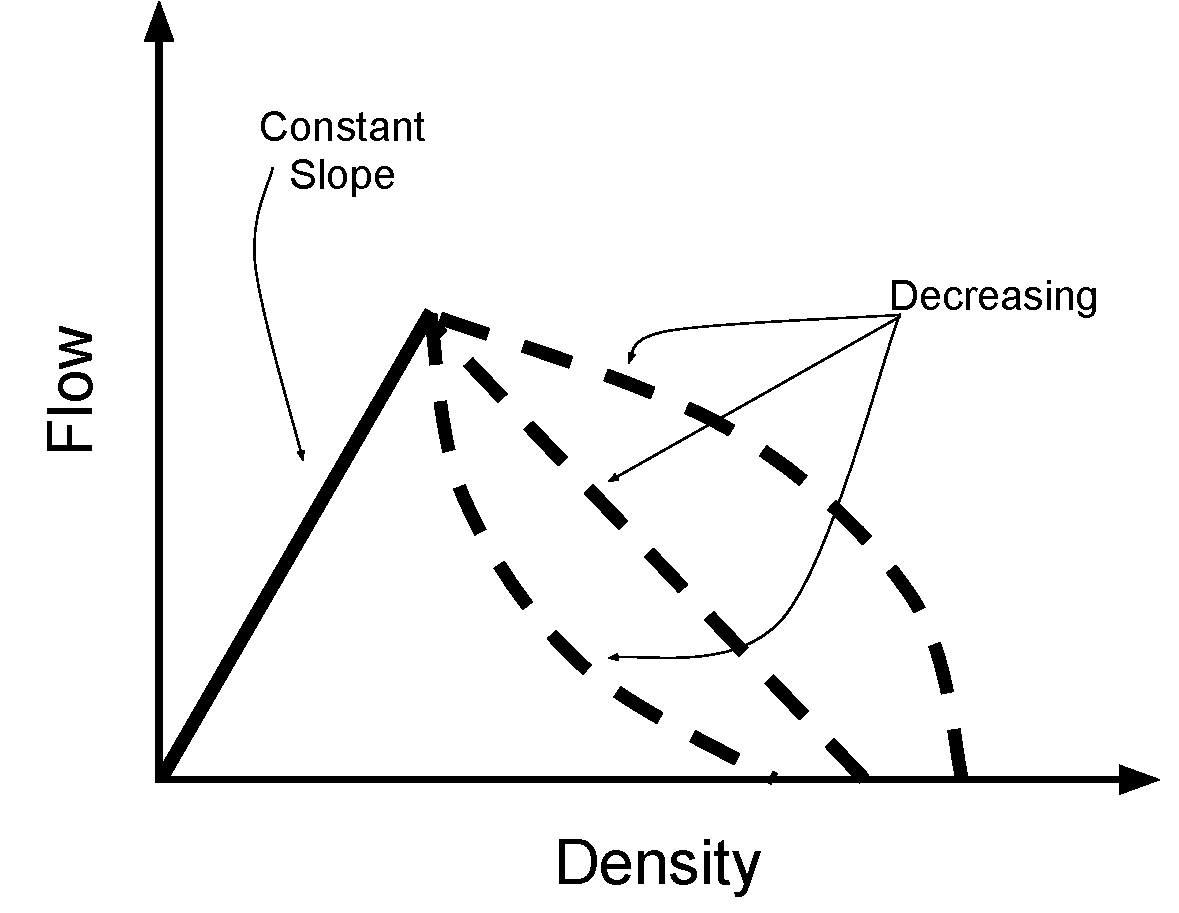
\includegraphics[scale=0.25]{../../figures/presentation/AnnotatedFundamentalDiagram}
\par\end{centering}
\caption{Class of fundamental diagrams considered}
\end{figure}



\end{frame}

%---------------------------------------------------------------------------------------------------------------------
\begin{frame}{Mapping to Latency}
\begin{itemize}
\item One-to-one mapping between density and latency.
\end{itemize}
\[
\latency[\mass]:\left[0,\massmax\right]\rightarrow\Rea[+]
\]

\begin{itemize}
\item Flow-to-latency mapping is not unique. Introduce a mode variable.
\end{itemize}
\[
\latency[\flow,\Mode]:\left[0,\flowMax\right]\times\left\{ 0,1\right\} \rightarrow\Rea[+]
\]


\begin{figure}
\subfloat[As function of density]{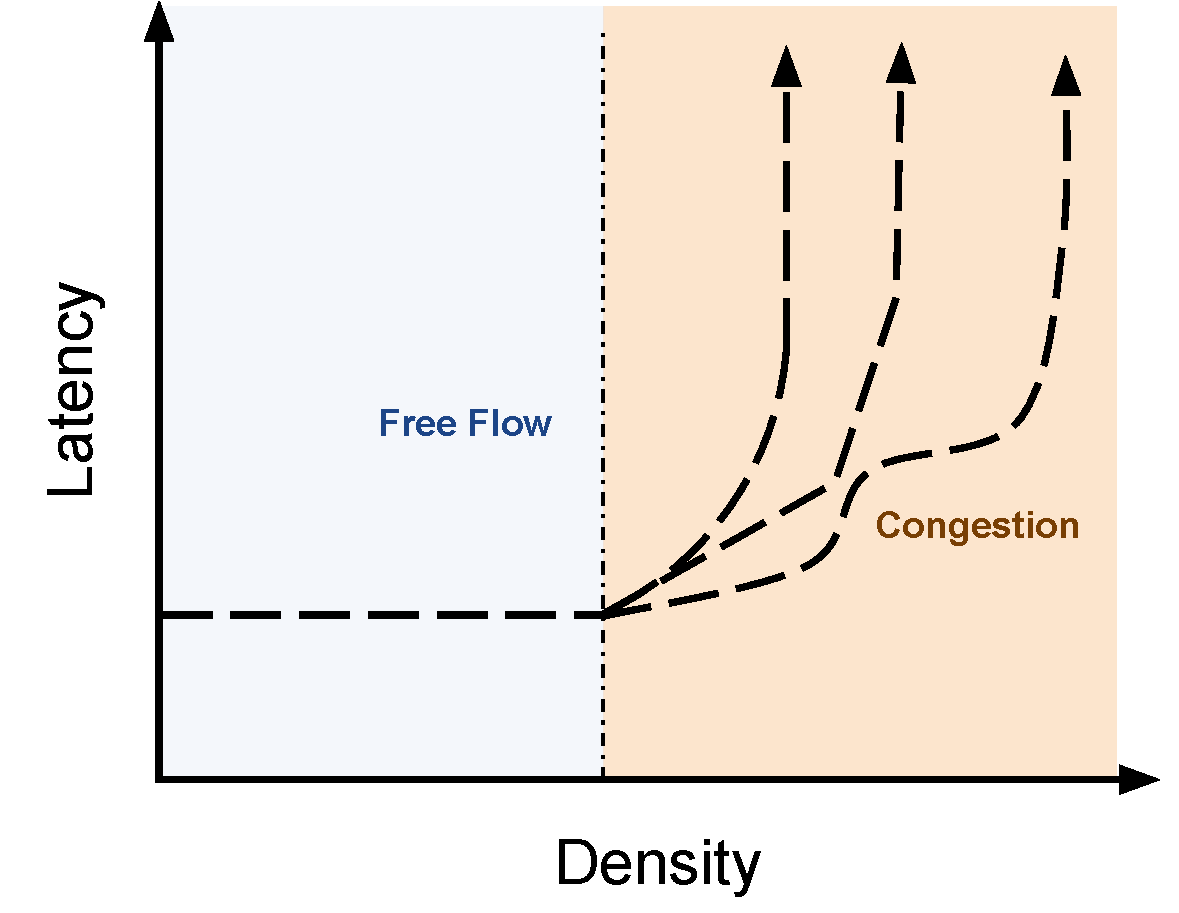
\includegraphics[scale=0.2]{../../figures/presentation/LatencyasFunctionofDensity}

}\subfloat[As function of density]{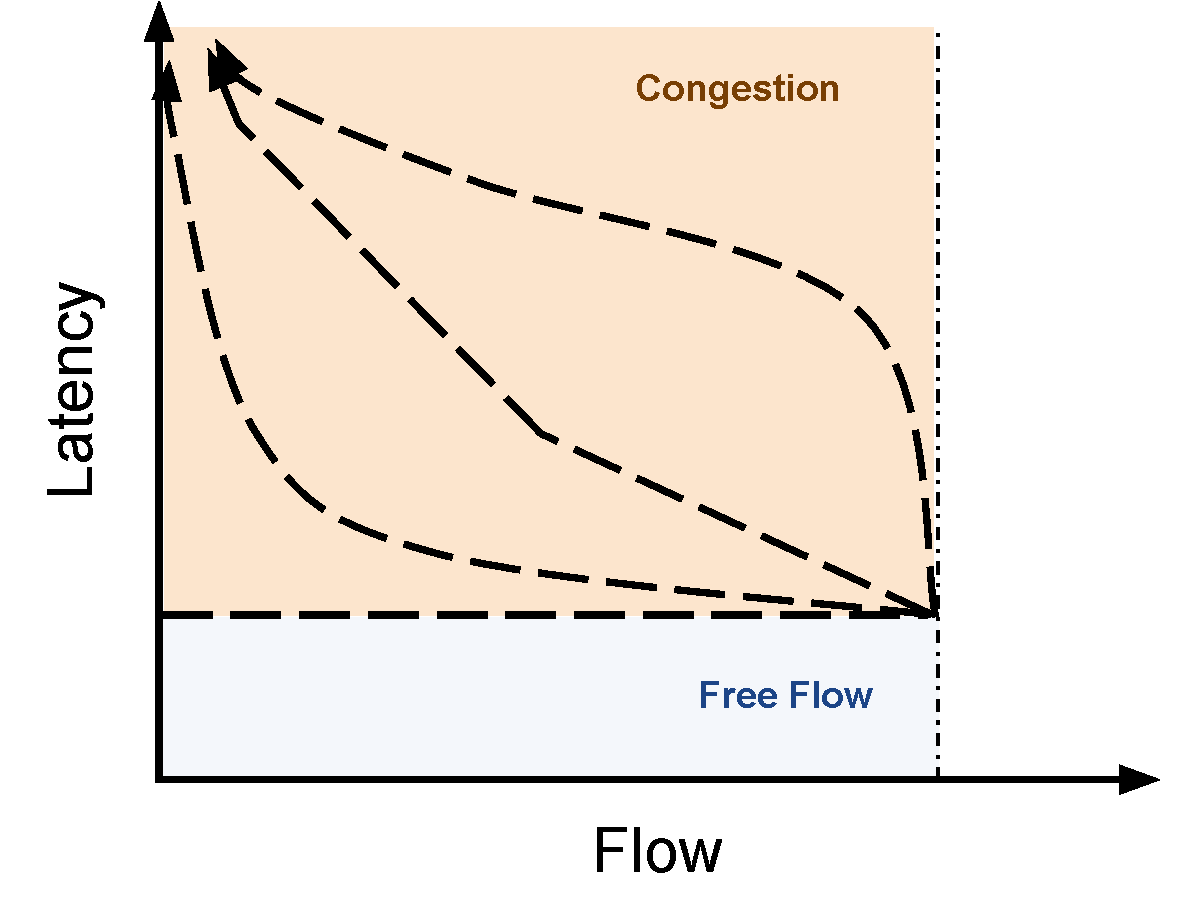
\includegraphics[scale=0.2]{../../figures/presentation/LatencyasFunctionofFlowMode}

}

\begin{centering}
\caption{Relating flow-density relationship to latency}

\par\end{centering}

\end{figure}



\end{frame}


\section{Nash Equilibria}

%###########################################################################################################
\subsection{Enumerating All Nash Equilibria}


\begin{frame}{Definition of NE}

	Informally, NE exists when there is no incentive for any flow to switch
from current link.
\begin{defn}
An assignment $\left(\flow,\Mode\right)\in\Rea[\NLinks]_{+}\times\left\{ 0,1\right\} ^{\NLinks}$
for a parallel network instance $\left(\NLinks,\qdemand\right)$ is
at Nash equilibrium, if $\forall\link:\flow[\link]>0\implies\latency[\link]\left(\flow[\link],\Mode[\link]\right)\le\latency[k]\left(\flow[k],\Mode[k]\right)$
\end{defn}
\begin{figure}
\begin{centering}
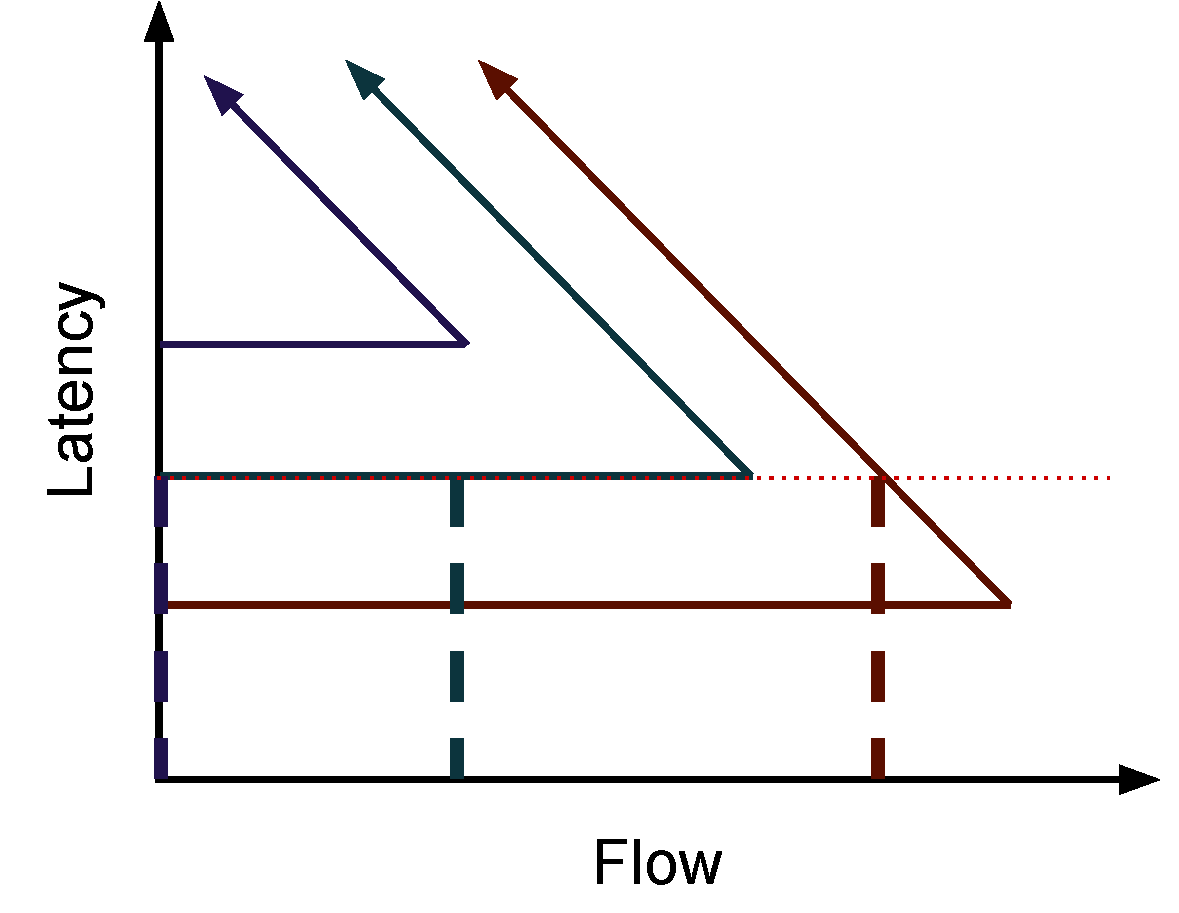
\includegraphics[scale=0.25]{../../figures/presentation/NE3link}
\par\end{centering}

\caption{An instance of a Nash equilibrium with one link in congestion, one
in free flow, and one unused}
\end{figure}



\end{frame}

%---------------------------------------------------------------------------------------------------------------------
\begin{frame}{Understanding Congestion Configuration}

For Nash equilibria, one can determine the congestion mode of a link
from the mode of other links.
\begin{lem}
\label{lem:filluplower}Let $\left(\flow,\Mode\right)\in\NashEquilibrium{\NLinks}{\qdemand}$.
Then $j\in\Supp{\flow}\implies\Mode[i]=1\quad\forall i\in\left\{ 1,\ldots,j-1\right\} $


\end{lem}
\begin{figure}
\begin{centering}
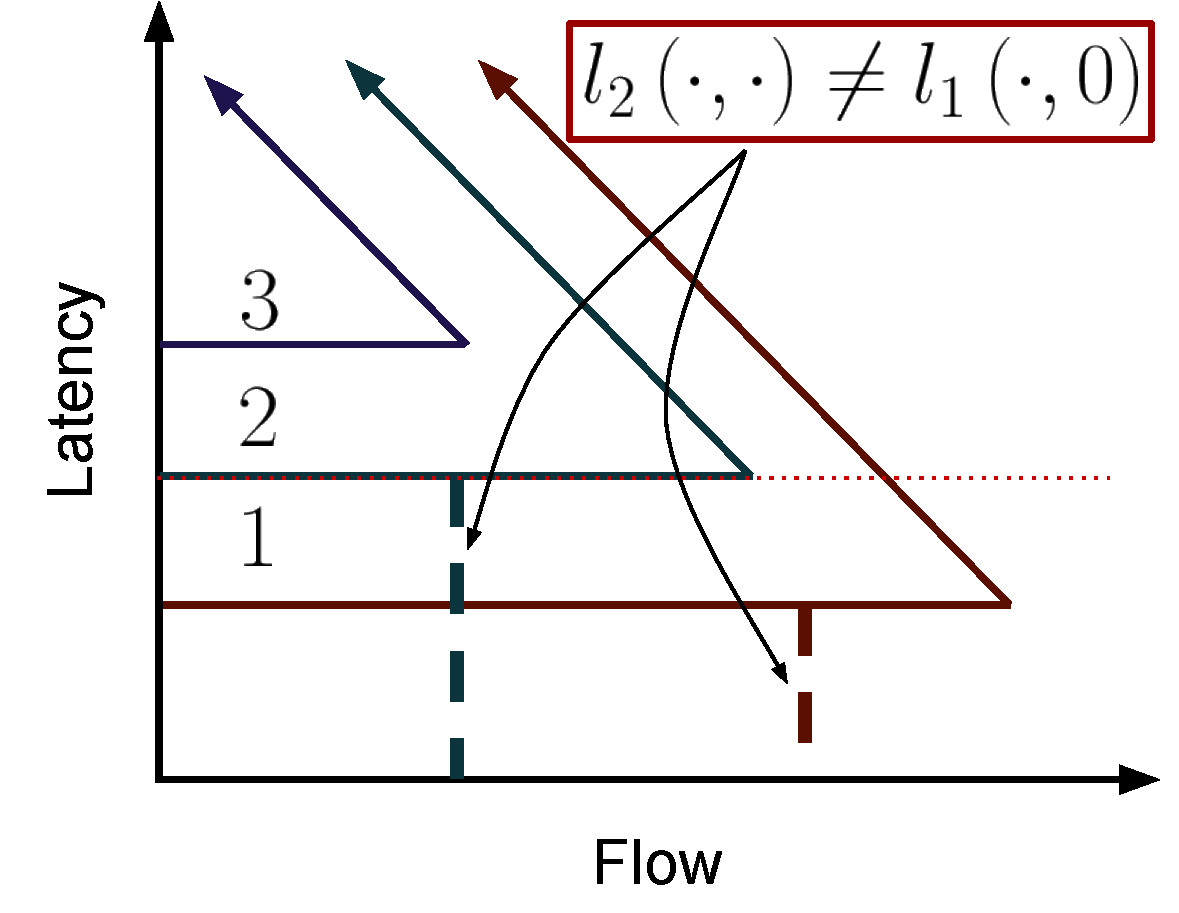
\includegraphics[scale=0.25]{../../figures/presentation/LemmaLowerIndexLinksCongested}
\par\end{centering}

\caption{If a link is utilized, then all links with lower free flow speed must
be congested.}
\end{figure}



\end{frame}

%---------------------------------------------------------------------------------------------------------------------
\begin{frame}{Understanding Congestion Configuration}

For NE, one can determine the congestion mode of a link from the mode
of other links.
\begin{cor}
Let $\left(\flow,\Mode\right)\in\NashEquilibrium{\NLinks}{\qdemand}$.
Assume that $\exists k\in\Supp{\flow}$ such that $m_{k}=0$. Then
$m=(1,\dots,\overset{k-1}{1},\overset{k}{0},\dots,0)$ and $\Supp{\flow}=\left\{ 1,\dots,k\right\} $.
\end{cor}
\begin{figure}
\begin{centering}
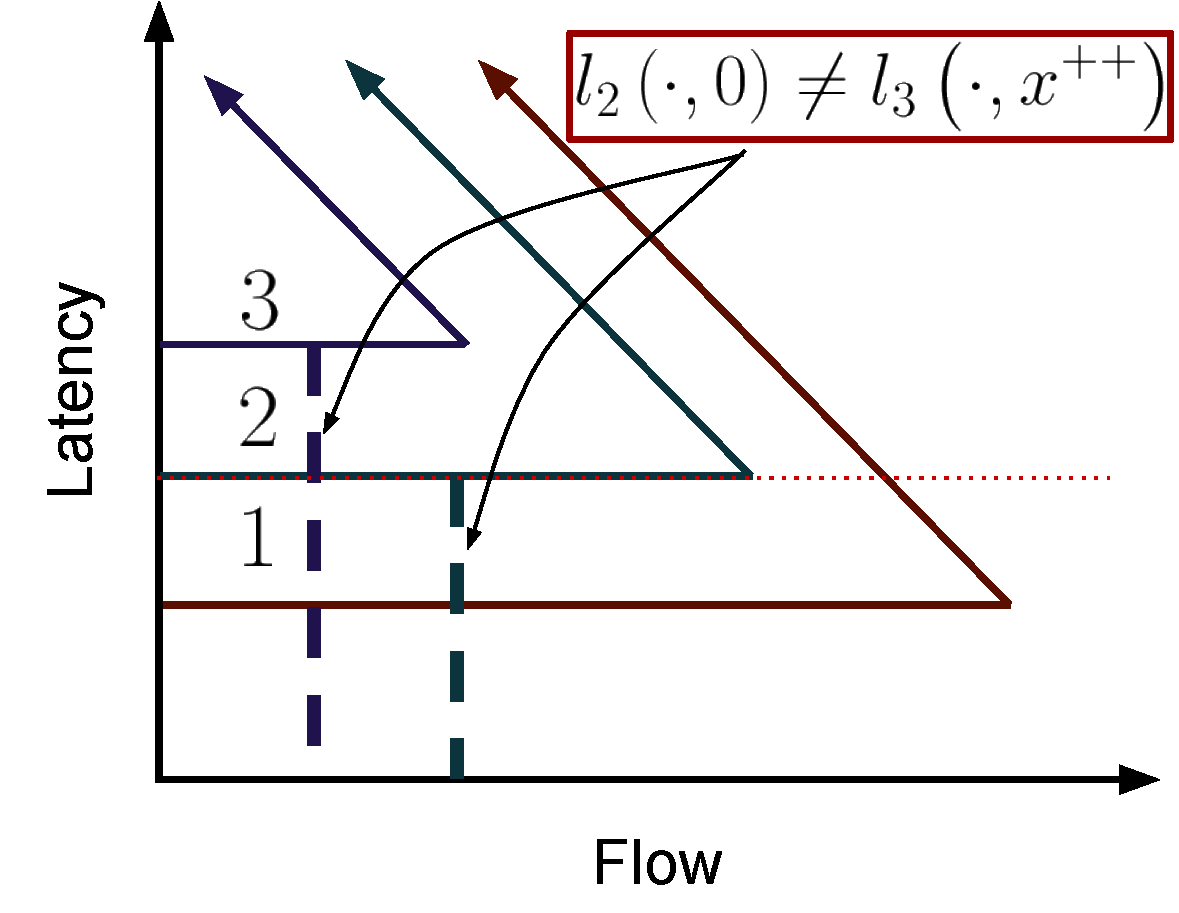
\includegraphics[scale=0.25]{../../figures/presentation/CorollaryAllaboveFFareempty}
\par\end{centering}

\caption{If a link is utilized and in free flow, then all links with higher
free-flow speeds must be empty}
\end{figure}



\end{frame}

%---------------------------------------------------------------------------------------------------------------------
\begin{frame}{Understanding Congestion Configuration}
\begin{itemize}
\item For NE, flows can be uniquely determined from the mode configuration. 
\item If we can enumerate mode config's, we can enumerate all NE.\end{itemize}
\begin{lem}
\label{lem:uniquemode}For a given congestion state $\Mode$, there
is at most one assignment $x$ such that $(x,m)$ is at Nash equilibrium.
\end{lem}
\begin{figure}
\begin{centering}
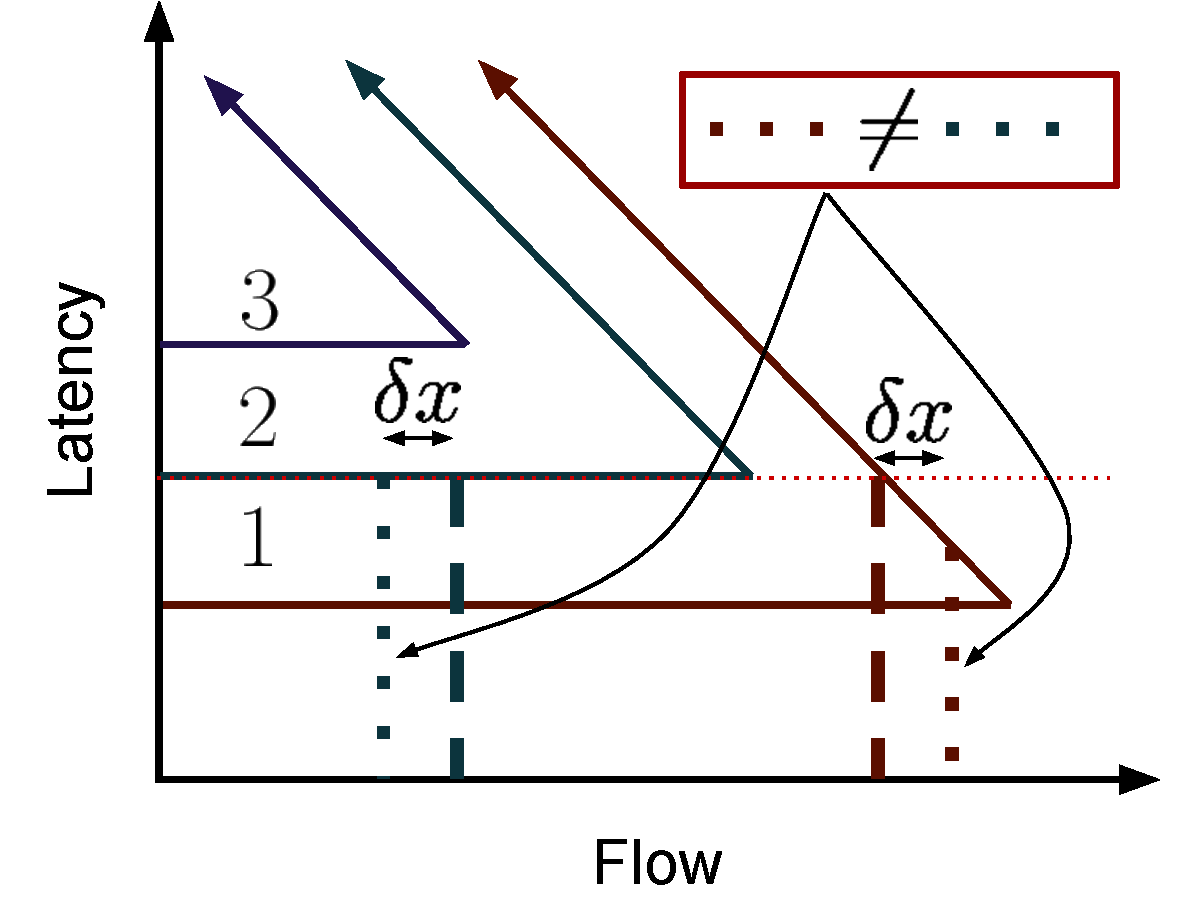
\includegraphics[scale=0.25]{../../figures/presentation/LemmaUniqueFlowFromMode}
\par\end{centering}

\caption{There may not exist two distinct Nash equilibria with the same congestion
state.}
\end{figure}



\end{frame}

%###########################################################################################################
\subsection{Existence of Uncongested Equilibrium}


\begin{frame}{Single-Link Free-Flow Nash Equilibria}
\begin{defn}
For $1\leq n<k\leq N$, congestion flow $\cffFlow nk$ is the unique
flow in $[0,\flowMax[n]]$ that satisfies

\[
l_{n}(\cffFlow nk,1)=a_{k}
\]

\end{defn}
\begin{figure}
\begin{centering}
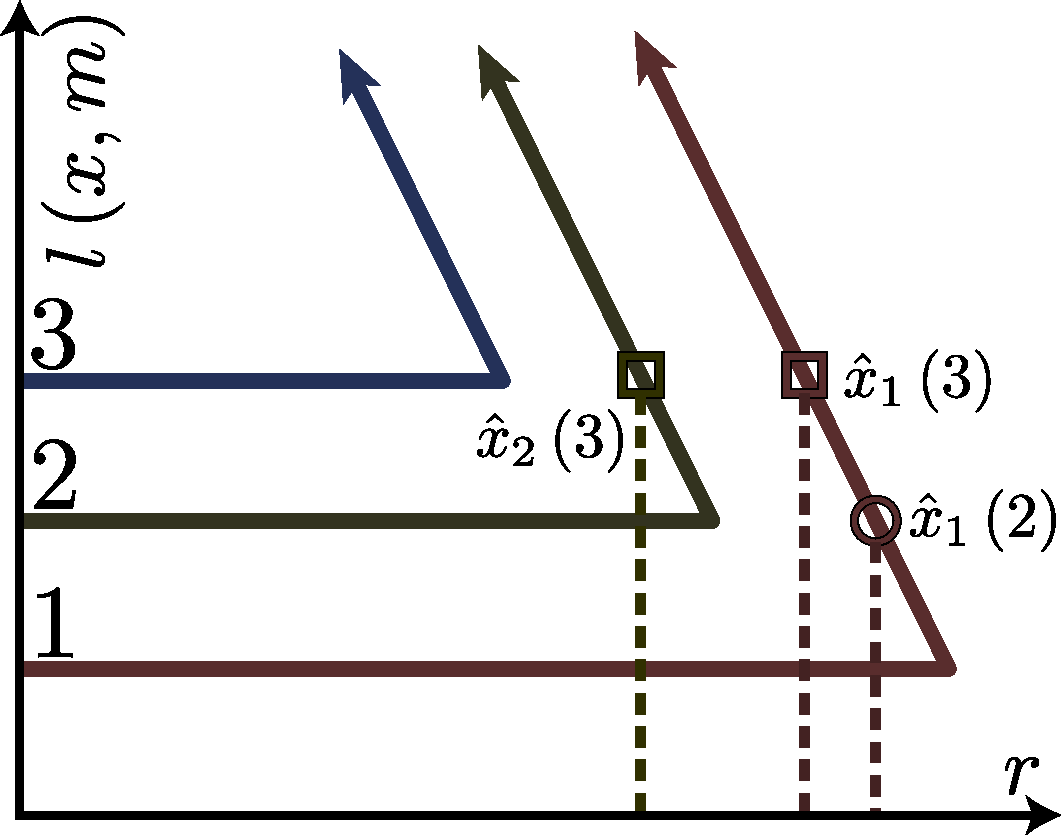
\includegraphics[scale=0.25]{../../figures/presentation/DefinitionXHat}
\par\end{centering}

\caption{Congested flows can be determined in reference to link in free-flow.}
\end{figure}



\end{frame}

%---------------------------------------------------------------------------------------------------------------------
\begin{frame}{Single-Link Free-Flow Nash Equilibria}
\begin{defn}

\begin{eqnarray*}
\bar{\Mode}^{k} & \coloneqq & (1,\dots,\overset{k-1}{1},\overset{k}{0},\dots,0)\\
\opneFlow k{\qdemand} & \coloneqq & (\cffFlow 1k,\dots,\overset{k-1}{\cffFlow{k-1}k}, r-\sum_{\link=1}^{k-1}\cffFlow{\link}k, 0, \dots, 0)
\end{eqnarray*}

\end{defn}

\begin{figure}
\subfloat[Link 3 free-flow NE]{\begin{centering}
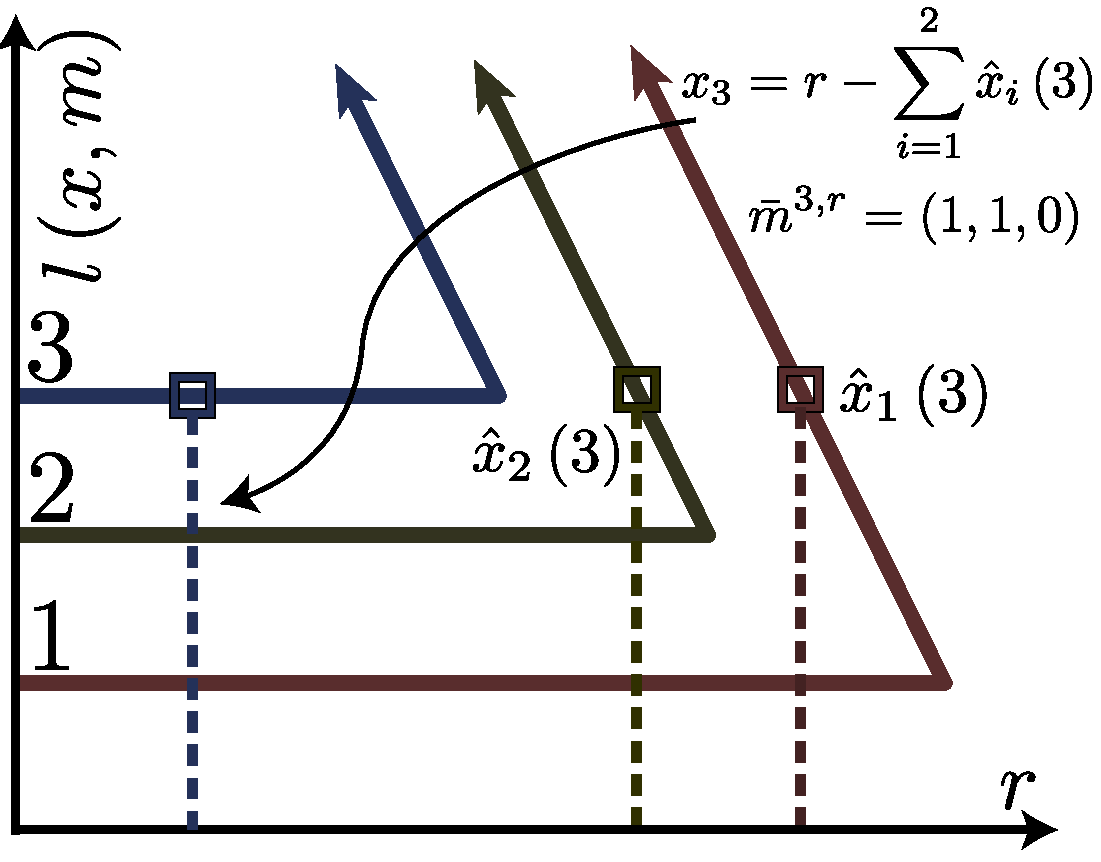
\includegraphics[scale=0.2]{../../figures/presentation/DefinitionXBar}
\par\end{centering}
}\subfloat[Completely congested NE]{\begin{centering}
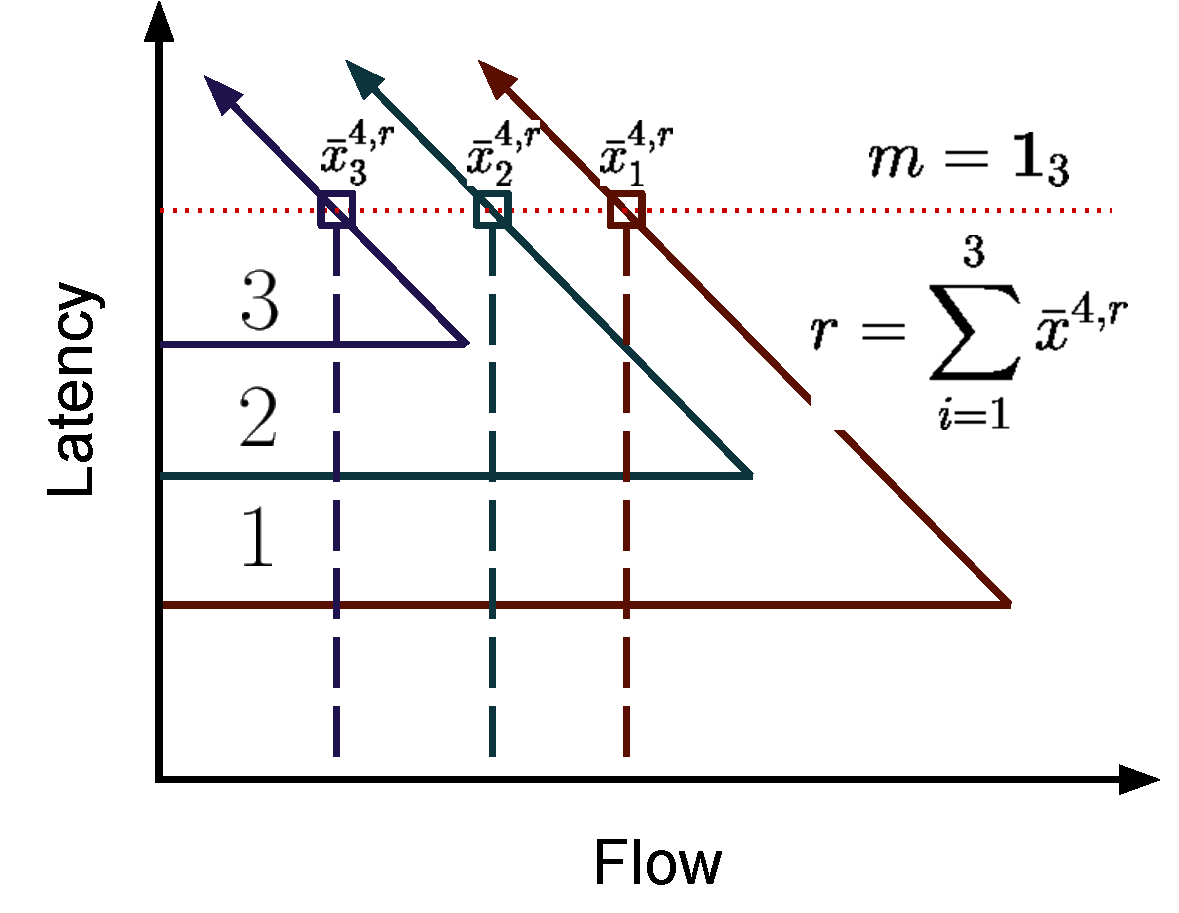
\includegraphics[scale=0.2]{../../figures/presentation/DefinitionCompletelyCongestedEquilibrium}
\par\end{centering}
}
\caption{Characterizing NE by mode configuration.}
\end{figure}


\end{frame}

%###########################################################################################################
\subsection{Best Nash Equilibrium}


\begin{frame}{Existence of Free Flow NE}

Completely congested NE is \textbf{never} only NE, can be used for
proving Best NE.
\begin{lem}
$\exists$ completely congested Nash equilibrium $\left(\flow,\cffMode{\NLinks+1}\right)\in\NashEquilibrium{\NLinks}{\qdemand}$ $\implies\exists$
free flow Nash equilibrium \textrm{\textup{$\left(\opneFlow j{\qdemand},\cffMode j\right)\in\NashEquilibrium{\NLinks}{\qdemand}$
for some $j\leq N$.}}
\end{lem}
By induction, proof iteratively seeks ``lower potential'', until
feasible mode config. found.

\begin{figure}
\begin{centering}
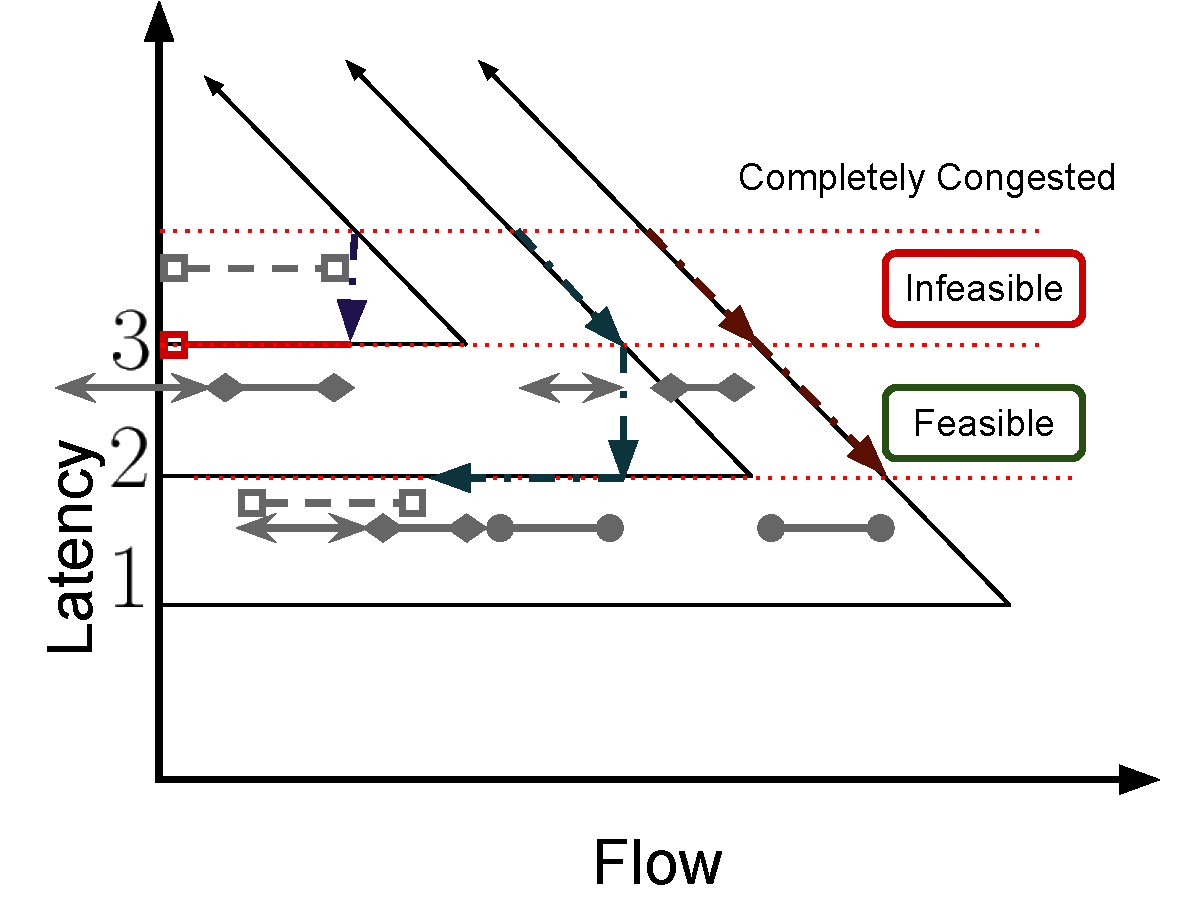
\includegraphics[scale=0.25]{../../figures/presentation/LemmaExistenceofSingleLinkFreeFlowNE}
\par\end{centering}

\caption{Illustration: $k=3$ infeasible, $k=2$ accommodates all flow.}
\end{figure}



\end{frame}

%---------------------------------------------------------------------------------------------------------------------
\begin{frame}{Best Nash Equilibrium}

The best NE for a network $\NLinks$ and demand $\qdemand$ is uniquely
expressed as the free-flow NE that utilizes the fewest links.

\begin{defn}
$\BestNashEquilibrium{\NLinks}{\qdemand}=\underset{\left(\flow,\Mode\right)\in\NashEquilibrium{\NLinks}{\qdemand}}{\arg\min}\Latency\left(\flow,\Mode\right)$
\end{defn}

\begin{figure}
\begin{centering}
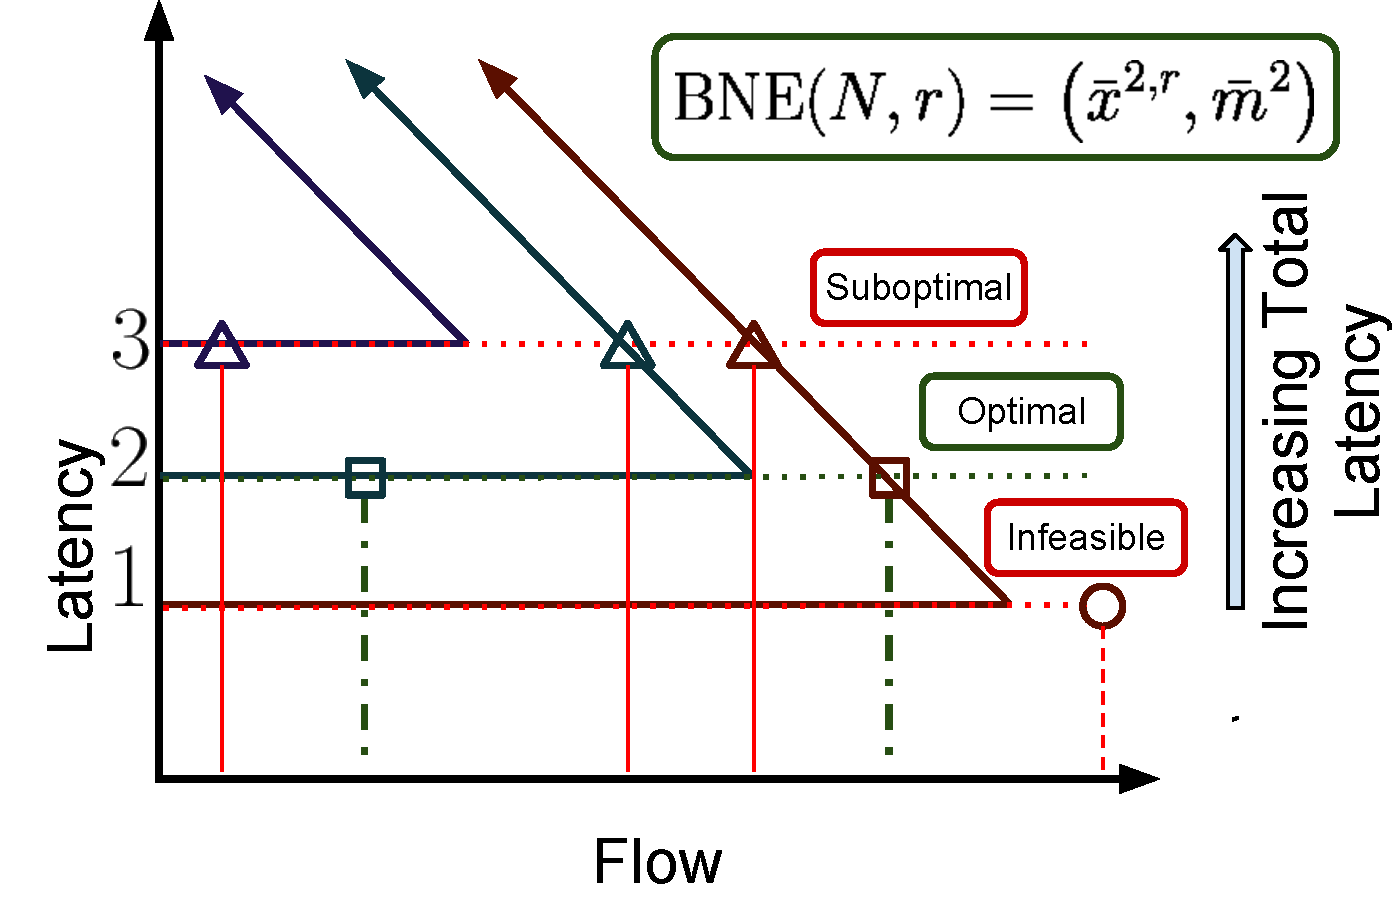
\includegraphics[scale=0.25]{../../figures/presentation/TheoremBestNashEquilibrium}
\par\end{centering}

\caption{The BNE occurs with $k=2$ in free-flow, as $k=1$ is infeasible,
and all others must be suboptimal.}
\end{figure}


\end{frame}

%###########################################################################################################
\subsection{Price of Stability}

%---------------------------------------------------------------------------------------------------------------------
\begin{frame}{Social Optimum}


\end{frame}



%###########################################################################################################
\section{Stackelberg Routing}

\subsection{Stackelberg Routing Game}

\begin{frame}{Stackelberg Routing Game}

\begin{itemize}
\item Stackelberg instance $(N, r, \beta)$
\item $\beta$ is the fraction of compliance
\item Leader: route compliant flow $\beta r$
\item Followers: choose their routes selfishly after Stackelberg strategy is revealed.
\end{itemize}


\begin{block}{Definition: Stackelberg strategy}
Assignment $s$ of compliant flow (feasible for the instance $(N,\beta r)$)
\end{block}

\begin{block}{Induced Nash Equilibrium}
$s$ induces assignment $(t(s), m(s))$ of non-compliant flow at Best Nash Equilibrium
\[
t_n(s)>0 \Rightarrow \forall k \leq N, l_n(s_n + t_n(s), m_n(s)) \leq l_k(s_k + t_k(s), m_k(s))
\]
(if $n$ is in the support of $t$, all other links have greater latency)
\end{block}

Set of Stackelberg strategies: $S(N, r, \beta)$

\end{frame}

%---------------------------------------------------------------------------------------------------------------------

\begin{frame}{Stackelberg routing}

\begin{lemma}
Induced Equilibrium is a single-link free-flow equilibrium.
\[
m(s)_{\max \text{Supp}(t(s))} = 0
\]
\end{lemma}

Follows from $(t(s), m(s))$ is at Nash Eq for the instance $(N,\beta r)$ and latencies
\begin{align*}
\tilde{l}_n: [0, x_n^{\max} - s_n]\times \{0,1\} & \rightarrow \mathbb{R}_+\\
(x_n,m_n) & \mapsto l_n(s_n+x_n,m_n)
\end{align*}
and Theorem 1.

\end{frame}

%---------------------------------------------------------------------------------------------------------------------
\begin{frame}{Optimal Stackelberg Strategy}

\begin{block}{Optimal Stackelberg strategy}
$s^*$ is an optimal strategy if the cost of the induced equilibrium
\[
C(s^* + t(s^*), m(s^*))
\]
is minimal over $S(N, r, \beta)$
\end{block}



\begin{block}{Stackelberg Equilibrium}
Equilibrium induced by an optimal Stackelberg strategy $s^*$.
\end{block}

\end{frame}


%###########################################################################################################
\subsection{Computing The Optimal Stackelberg Strategy}

\begin{frame}{Computing the Optimal Stackelberg Strategy}

\begin{block}{Non-Compliant First strategy $\bar{s}$}
\begin{itemize}
\item \alert<3>{Compute BNE of non-compliant users alone: $(\bar{t}, \bar{m}) = \text{BNE}(N, (1-\beta)r)$}
\item Compute $\bar{s}$: Assign the compliant flow by filling remaining links (non congested by non-compliant) each to max capacity.
\end{itemize}
\end{block}

\pause 
Intuitive argument
\begin{itemize}
\item $(\bar{t}, \bar{m})$ has best cost for non-compliant, cannot do better.
\item Best we can do with compliant users is assign them optimally so they do not ``degrade'' equilibrium $(\bar{t}, \bar{m})$
\end{itemize}


\end{frame}



%---------------------------------------------------------------------------------------------------------------------
\begin{frame}{Non-Compliant First}

\begin{figure}
\centering
\only<1>{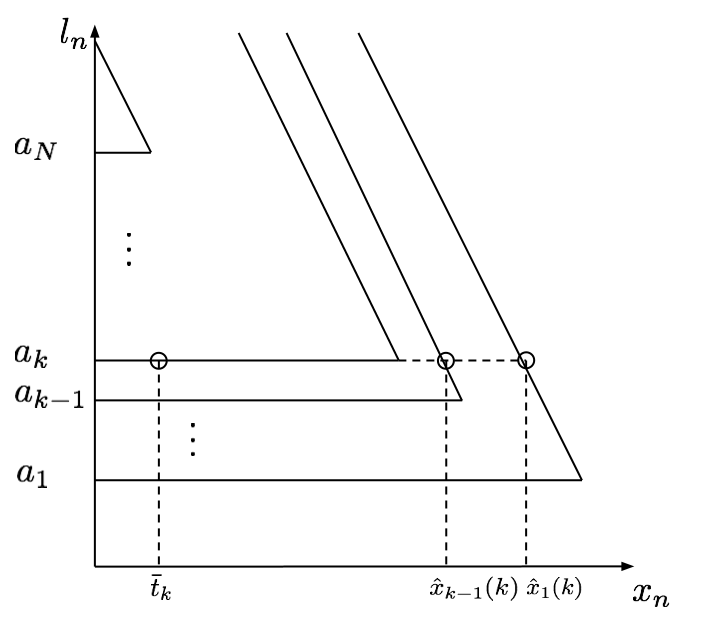
\includegraphics[scale=0.25]{../../figures/presentation/optimal_stackelberg1.png}}
\only<2>{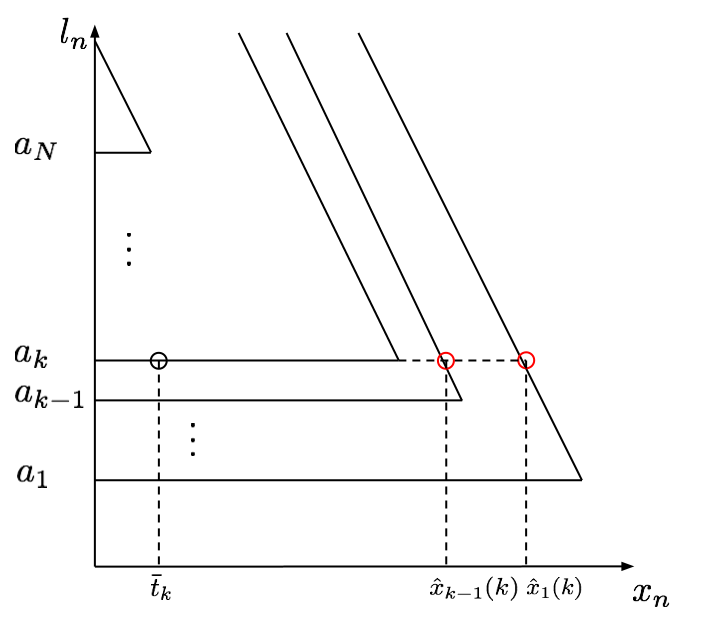
\includegraphics[scale=0.25]{../../figures/presentation/optimal_stackelberg1-1.png}}
\only<3>{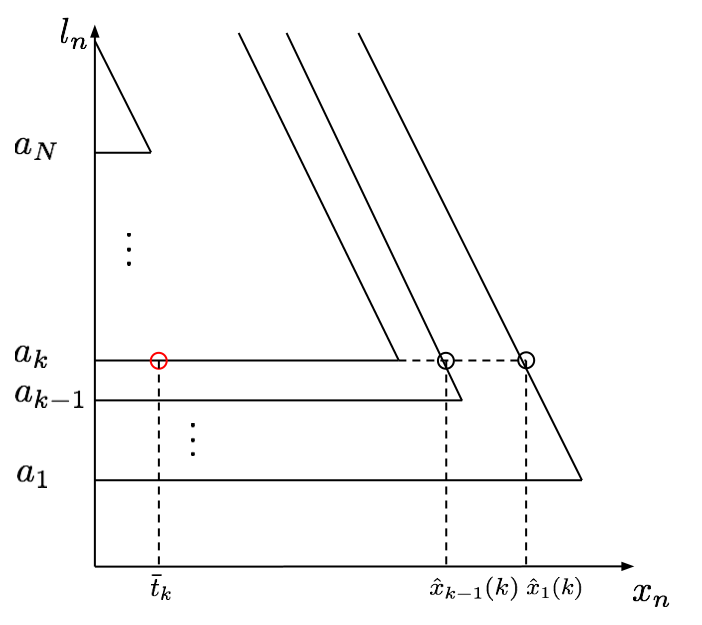
\includegraphics[scale=0.25]{../../figures/presentation/optimal_stackelberg1-2.png}}
\caption{Nash Equilibrium $(\bar{t}, \bar{m})$ of non compliant flow $(1-\beta)r$}
\end{figure}

\vskip-2ex 
\footnotesize

\begin{align*}
\bar{m} = (
\textcolor<2>{red}{1, \dots, 1}, 
\textcolor<3>{red}{\overset{k}{0}}, 
\dots, 0) 
&&
\bar{t} = \left( 
\textcolor<2>{red}{\hat{x}_1(k), \dots, \hat{x}_{k-1}(k)}, 
\textcolor<3>{red}{(1-\beta)r - \sum_{n = 1}^{k-1}\hat{x}_n(k)}, 
0, \dots, 0
\right)
\end{align*}


\end{frame}

%---------------------------------------------------------------------------------------------------------------------
\begin{frame}{Non-Compliant First}

\begin{block}{Non-Compliant First strategy $\bar{s}$}
\begin{itemize}
\item Compute BNE of non-compliant users alone: $(\bar{t}, \bar{m}) = \text{BNE}(N, (1-\beta)r)$
\item \alert{Compute $\bar{s}$: Assign the compliant flow by filling remaining links (non congested by non-compliant) each to max capacity.}
\end{itemize}
\end{block}

Intuitive argument
\begin{itemize}
\item $(\bar{t}, \bar{m})$ has best cost for non-compliant, cannot do better.
\item Best we can do with compliant users is assign them optimally so they do not ``degrade'' equilibrium $(\bar{t}, \bar{m})$
\end{itemize}


\end{frame}


%---------------------------------------------------------------------------------------------------------------------
\begin{frame}{Non-Compliant First}

\begin{figure}
\centering
\only<1>{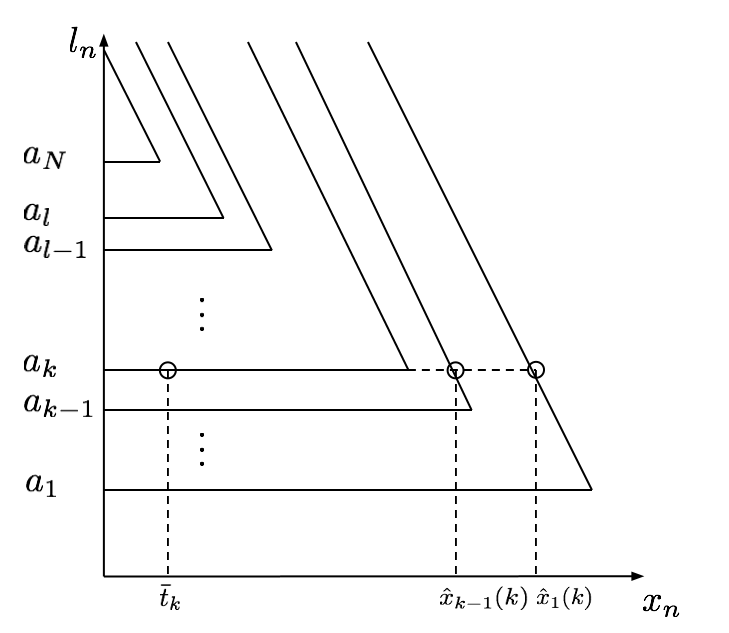
\includegraphics[scale=0.25]{../../figures/presentation/optimal_stackelberg2.png}}
\only<2>{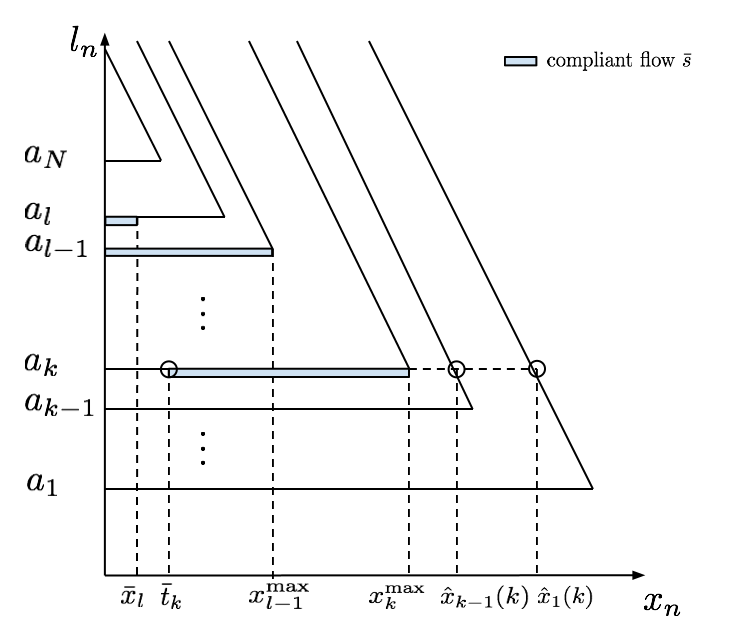
\includegraphics[scale=0.25]{../../figures/presentation/optimal_stackelberg3.png}}
\only<3>{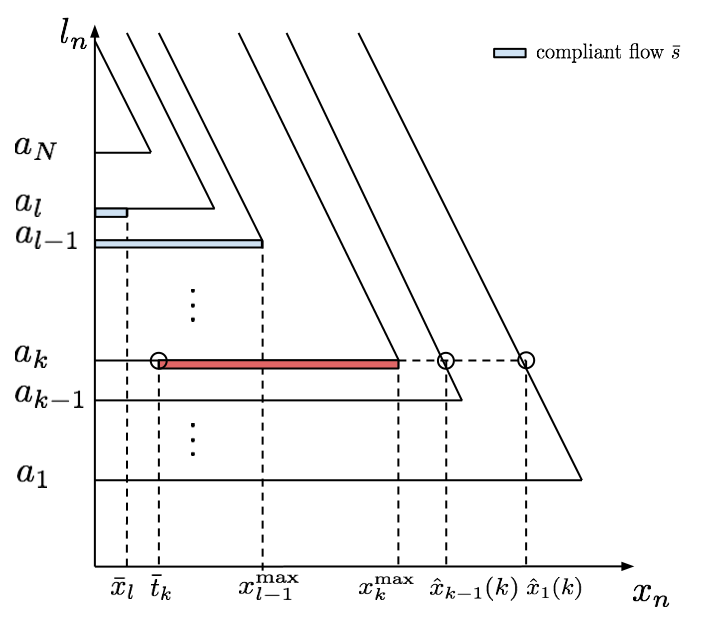
\includegraphics[scale=0.25]{../../figures/presentation/optimal_stackelberg3-1.png}}
\only<4>{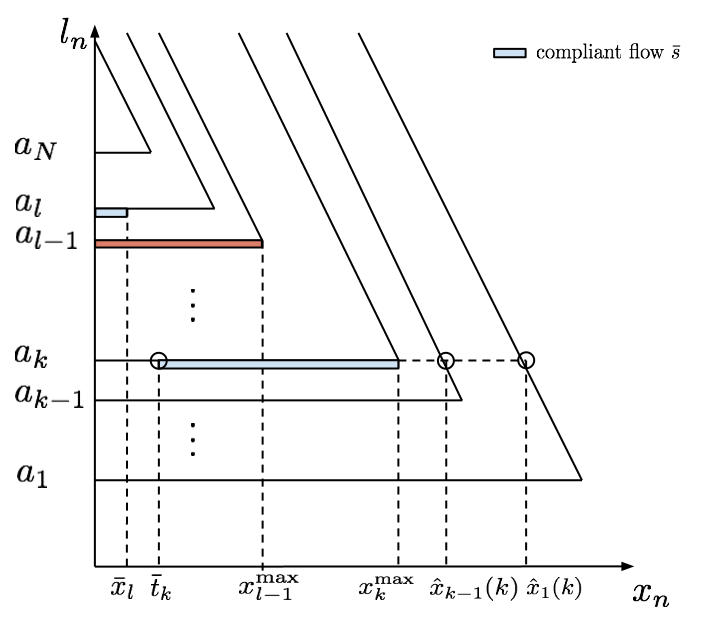
\includegraphics[scale=0.25]{../../figures/presentation/optimal_stackelberg3-2.png}}
\only<5>{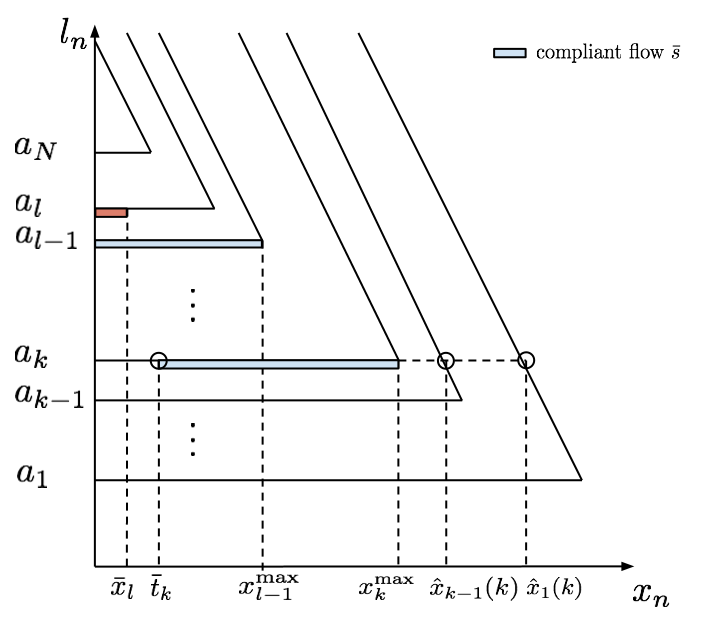
\includegraphics[scale=0.25]{../../figures/presentation/optimal_stackelberg3-3.png}}
\caption{Constructing the candidate strategy $\bar{s}$}
\end{figure}

\vskip-2ex 

\visible<2->{
\begin{align*}
\bar{s} = 
\left( 
0, \dots, \overset{k-1}{0}, 
\textcolor<3>{red}{ x_k^{\max} - \bar{t}_k}, 
\textcolor<4>{red}{x_{k+1}^{\max}, \dots, x_{l-1}^{\max}}, 
\textcolor<5>{red}{\beta r - (\sum_{n = k}^{l-1}x_n^{\max} - t_k)}, 
\overset{l}{0}, \dots, 0
\right)
\end{align*}
}

\end{frame}



%---------------------------------------------------------------------------------------------------------------------
\begin{frame}{Non-Compliant First is optimal}

Consider Stackelberg strategy $s$ and induced assignment $(t(s), m(s))$.\\
We want to show
\[
C(s+t(s), m(s)) \geq C(\bar{s} + \bar{t}, \bar{m})
\]

\vskip-2ex 

\begin{columns}[t]
\column{.4\textwidth}
\begin{figure}
\centering
\only<1>{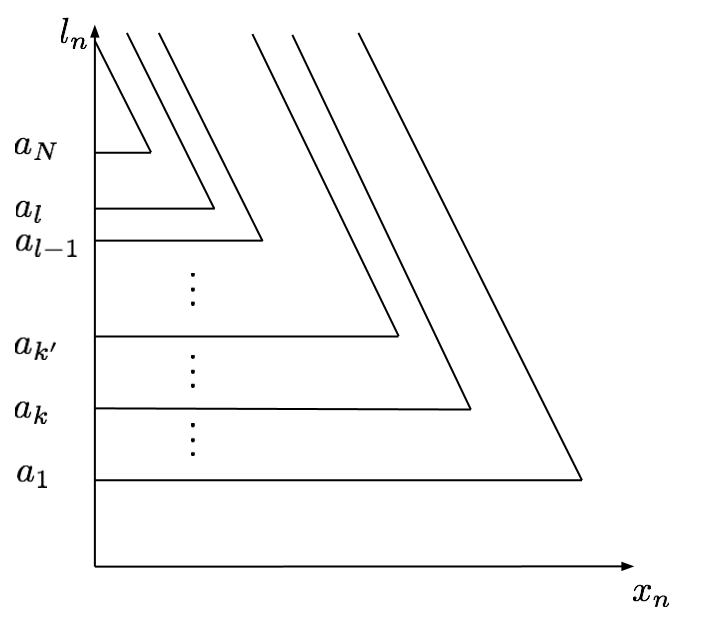
\includegraphics[scale=0.2]{../../figures/presentation/optimal_stackelberg_proof0.png}}
\only<2>{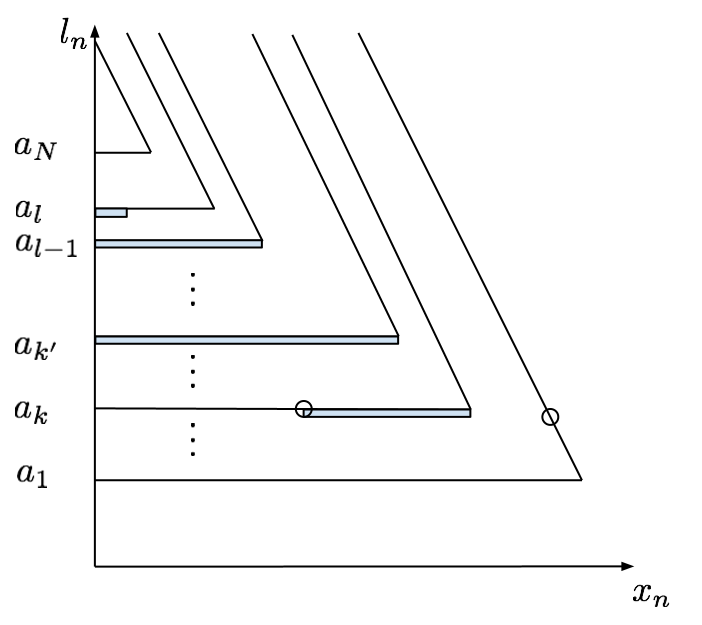
\includegraphics[scale=0.2]{../../figures/presentation/optimal_stackelberg_proof1.png}}
\only<3->{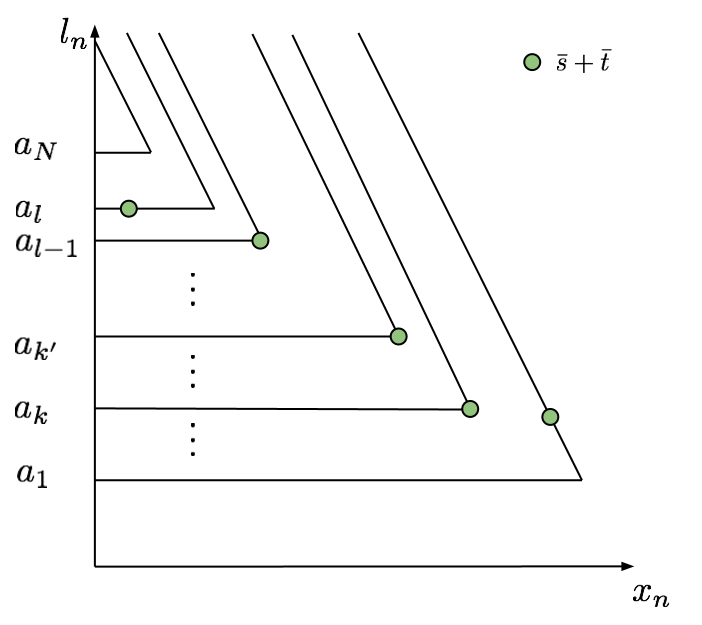
\includegraphics[scale=0.2]{../../figures/presentation/optimal_stackelberg_proof2.png}}
\caption{Assignment $\bar{s}+\bar{t}$}
\end{figure}


\column{.4\textwidth}
\begin{figure}
\centering
\only<1-3>{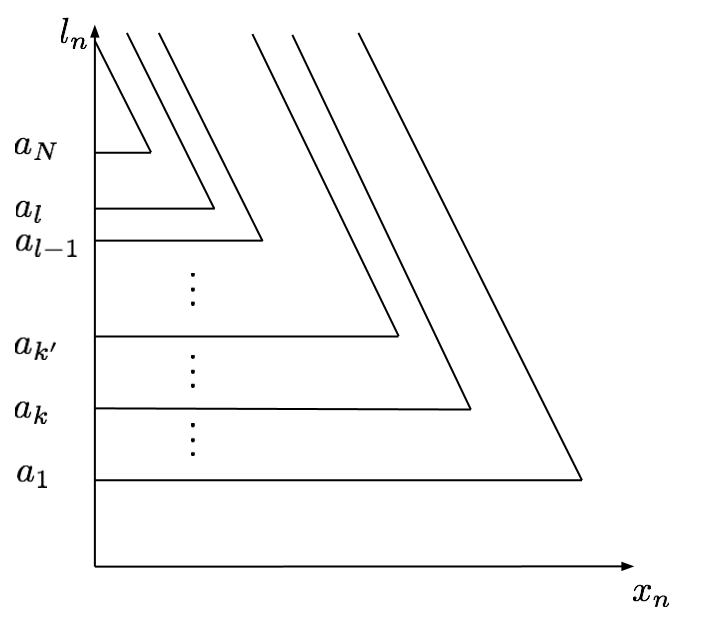
\includegraphics[scale=0.2]{../../figures/presentation/optimal_stackelberg_proof0.png}}
\only<4>{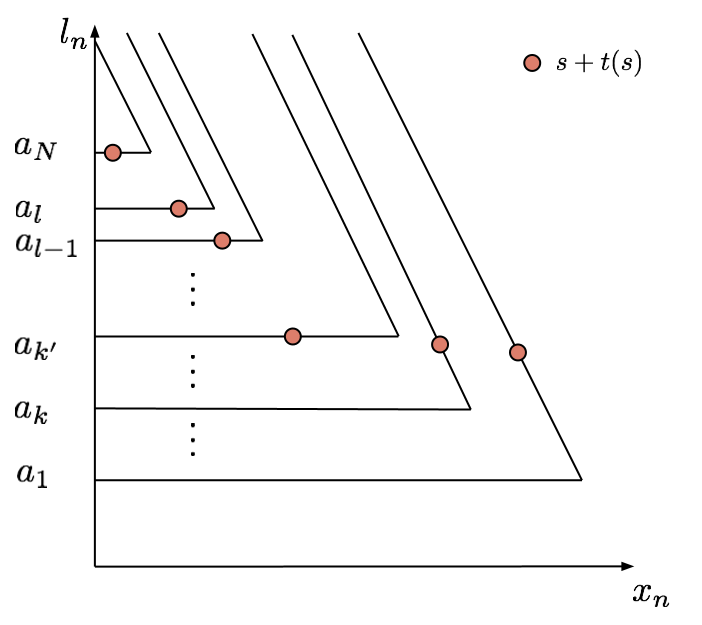
\includegraphics[scale=0.2]{../../figures/presentation/optimal_stackelberg_proof3.png}}
\caption{Assignment $s+t(s)$}
\end{figure}

\end{columns}

\end{frame}

%---------------------------------------------------------------------------------------------------------------------
\begin{frame}{Non-Compliant First is optimal}

Let $k = \max \text{Supp}(\bar{t})$ and $k = \max \text{Supp}(t)$
\begin{lemma}
$k' \geq k$
\end{lemma}


otherwise
\begin{itemize}
\item we can construct a Nash Equilibrium with support $\subset \{ 1, \dots, k'\}$ for the instance $(N, (1-\beta)r)$ (note that $\sum_{n\in \text{Supp}(t(s))} (s+t(s))_n \geq (1-\beta)r$)\\
\item \pause cost of this Equilibrium: $(1-beta r)a_{k'} < (1-beta r)a_k = C(\bar{t}, \bar{m})$
\item \pause contradicts definition of $(\bar{t}, \bar{m})$
\end{itemize}

\end{frame}


%---------------------------------------------------------------------------------------------------------------------
\begin{frame}{Non-Compliant First is optimal}

\begin{columns}[t]

\column{.5\textwidth}


\begin{figure}
\centering
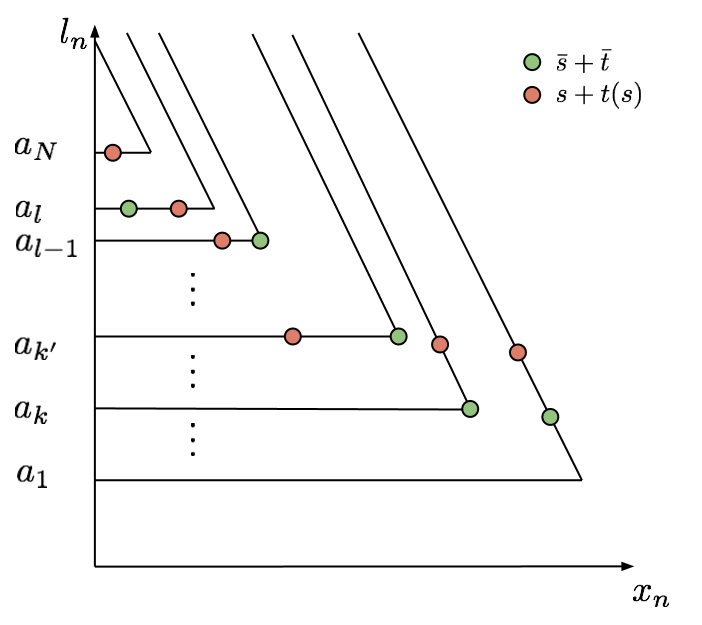
\includegraphics[scale=0.25]{../../figures/presentation/optimal_stackelberg_proof4.png}
\caption{Assignments $\bar{s}+\bar{t}$ and $s+t(s)$}
\end{figure}


\column{.4\textwidth}
\\[.7in]
We have $\forall n \in \{1, \dots, l-1\}$

\begin{itemize}
\item $l_n((s+t(s))_n) \geq l_n((\bar{s}+\bar{t})_n)$
\item $(s+t(s))_n \leq (\bar{s}+\bar{t})_n$
\end{itemize}

\end{columns}

\end{frame}



%---------------------------------------------------------------------------------------------------------------------
\begin{frame}

\large
\begin{center}
Thank you.
\end{center}
\end{frame}

\end{document}
